\documentclass{llncs}
\usepackage[T1]{fontenc}
\usepackage{graphicx}
\usepackage[inline]{enumitem}
\usepackage{amsmath}
\usepackage{listings}
\usepackage{tikz}
\usepackage{epstopdf}
\usepackage{multirow}
\usepackage{todonotes}
\usepackage{pifont}

\lstset{
  numbers=left,
  numberstyle=\tiny\ttfamily\color{black!40},
}

\lstdefinestyle{code}{
  basicstyle=\ttfamily\scriptsize,
  commentstyle=\color{black!50},
  classoffset=0,
  morecomment=[l]{\#},
  keywordstyle=\color{magenta!70!black!80},
  morekeywords={mov,movb,movzx,lfence,movl,shlx,jrcxz,lea,shrx,shlx,call,jmp,incl},
}

\title{Evaluating the Effectiveness of AEX-Notify against SGX Single-Stepping Attackers}
\author{Wicked Wench}
\institute{	University of L\"ubeck, Germany}
% TODO: For the camera-ready submission
%\author{Basil Ugbomoiko\inst{1} \quad Daniel Knaack\inst{1}}
%\institute{	University of L\"ubeck, Germany\\
%	\email{\{basil.ugbomoiko,daniel.knaack\}@student.uni-luebeck.de}}

\begin{document}

\maketitle

\begin{abstract}
  Trusted execution environments (TEEs) like Intel's Software Guard Extensions
  (SGX) offer a promising avenue for securing applications by executing them
  within secure enclaves.
  However, recent advancements in side-channel attack techniques, such as
  SGX-Step, pose significant threats to the security guarantees provided by
  SGX.
  SGX-Step uses the APIC timer to precisely interrupt the enclave after each
  instruction, effectively stepping through the execution one instruction at a
  time.
  These single-stepping capabilities allow for a higher time resolution,
  thereby enhancing the feasibility of side-channel attacks.
  In response to this threat, AEX-Notify has been proposed as a potential
  mitigation against SGX-Step. AEX-Notify is both a hardware extension and a
  software mitigation that tries to prevent adversaries from single-stepping
  enclaves.
  This paper analyzes the security of AEX-Notify and evaluates its
  effectiveness against deterministic single-stepping.
\end{abstract}

\section{Motivation}

Modern computing relies heavily on privileged system software to manage
interactions and ensure security.
However, traditional operating system kernels are susceptible to bugs and
vulnerabilities due to their large codebase written in unsafe languages.
To address this, recent research has focused on Protected Module Architectures
(PMAs), aiming to support isolated execution of security-sensitive components
called enclaves with minimal Trusted Computing Base (TCB).
Intel’s Software Guard eXtensions (SGX) \cite{Intel16,Intel17} represent a
significant advancement, providing hardware-enforced trusted computing
guarantees.
However, vulnerabilities have emerged, particularly in information leakage
through attacks exploiting various system components.
These vulnerabilities undermine the security promises of SGX.

SGX-Step \cite{BulckPS17} presents a novel framework to address SGX vulnerabilities by enabling
precise monitoring of enclave execution at the instruction level.
Unlike previous methods, SGX-Step achieves true single-stepping for any enclave
program, significantly enhancing the resolution of existing attacks.
The framework comprises a Linux kernel driver and a runtime library, providing
the means to interrupt enclave execution at the instruction level for detailed
observation and analysis.

For Intel SGX enclaves, AEX-Notify is a security feature that prevents
single-stepping attacks such as SGX-Step \cite{ConstableBCXXAK23}. Enclaves can
react to possible threats by using the ability to recognize Asynchronous
Enclave eXit (AEX) events.
AEX-Notify introduces a notification mechanism for Asynchronous Enclave Exits
(AEX) events within Intel SGX enclaves.
AEX events occur when the processor interrupts the execution of an enclave to
handle external events such as interrupts or exceptions.
These interruptions can be exploited by attackers to perform timing attacks or
manipulate the control flow of the enclave.

The main mechanism of AEX-Notify involves detecting AEX events and notifying
the enclave when they occur.
Upon receiving this notification, the enclave can take defensive actions to
protect sensitive information.
These actions may include deleting sensitive data or resetting execution states
to ensure that no critical information is exposed during the interruption.

The primary advantage of AEX-Notify lies in its ability to improve the security
of the enclave by disrupting the precise timing required for certain types of
attacks.
By enabling enclaves to verify their state upon resumption and apply adaptive
security measures, AEX-Notify helps maintain the integrity of the execution
environment.
This increases the resilience of the enclave against various interruption-based
threats, thereby enhancing overall security.

This paper attempts to evaluate the effectiveness of AEX-Notify in mitigating
single-stepping attacks against SGX enclaves.
Specifically, we have tested AEX-Notify on an attacker implementation and have
compared the ability to single-step with and without AEX-Notify enabled.
We have used the results from our tests to analyze AEX-Notify and find
potential weak points in its implementation.
Additionally, we have tested these weak points to see if an attack against
AEX-Notify is feasible or whether AEX-Notify still prevents single-stepping.

\section{Background}

This section provides an overview of Intel Software Guard Extensions (SGX) and
the mechanism of Asynchronous Enclave Exits (AEX).
We discuss the basic workings of Intel SGX, which enables the creation of
secure enclaves that protect the confidentiality and integrity of the data and
code within them, even from higher-privileged software such as the operating
system.

\subsection{Intel SGX}

The main feature behind Intel SGX are enclaves, that attempt to provide a
secure environment for safety-critical applications.
SGX ensures that the memory of an enclave cannot be accessed from the outside
world even by an untrusted operating system.
However, it still leaves the page tables under explicit control of the
operating system.
This means, for example, that the OS can modify the Page-Table Entries (PTEs),
specifically the present (P), accessed (A) and dirty (D) bit.

\newcommand\greenbox[1]{\tikz[baseline=(a.base)]\protect\node[enumerate] (a) {#1};}

\tikzset{enumerate/.style={draw, thick, green!70!black, font=\sffamily\scriptsize, inner sep=2pt}}
\begin{figure}
  \centering
  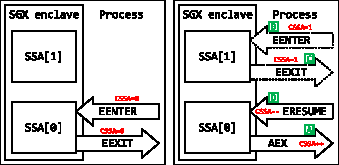
\includegraphics[width=0.6\textwidth]{images/sgx-ssa.pdf}
  \caption{Behavior of \textsc{eenter} and \textsc{eresume} \cite{ConstableBCXXAK23}.
    After an AEX occurs, the \textsc{cssa} field is incremented \protect\greenbox{A},
    such that the next \textsc{eenter} \protect\greenbox{B} and \textsc{eexit} \protect\greenbox{C} instructions use a different SSA.
    \textsc{eresume} decrements the \textsc{cssa} field again \protect\greenbox{D}
    and resumes the original enclave.}
  \label{fig:sgx-ssa}
\end{figure}

The operating system also has control over the execution of the enclave.
The main structure that controls the execution of an enclave is the Thread
Control Structure.
A thread can enter an enclave by calling the \textsc{eenter} instruction and
providing an address to one such TCS.
The enclave can be exited by calling the \textsc{eexit} instruction.
During the execution of an enclave, the operating system has the ability to
interrupt the enclave, for example by inducing a page-fault.
This causes an Asynchronous Enclave Exit (AEX) to occur, which is similar to a
context switch for normal processes.
The procedure saves the register state in a State Save Area (SSA) inside the
enclave.
This state is later restored once the enclave is resumed using the
\textsc{eresume} instruction.
More specifically, the TCS has a \textsc{cssa} field that indicates the index
of the current SSA.
After an AEX, this value is incremented, such that a new enclave will use a
different SSA, and after resuming the enclave, this value is decremented again.
Figure~\ref{fig:sgx-ssa} illustrates this process.

\section{Related Work}

This section provides a comprehensive review of existing research and
frameworks relevant to the evaluation of AEX-Notify against SGX single-stepping
attackers.
In particular, we discuss how SGX-Step leverages the APIC timer to single-step
enclaves.
Following this, we examine CopyCat, which leverages SGX-Step to extract
control-flow information from enclaves, highlighting potential security
vulnerabilities.
Finally, we look into the details of AEX-Notify and how it prevents the
single-stepping capabilities of SGX-Step.

\subsection{SGX-Step}

SGX-Step \cite{BulckPS17} is a framework that enhances the ability to monitor
SGX enclave execution at the instruction level, addressing vulnerabilities by
enabling precise and detailed observation.
It uses a timer from the Advanced Programmable Interrupt Controller (APIC) to
interrupt enclave execution at specific intervals.
This approach overcomes previous challenges related to time jitter by
configuring the timer in user space, which allows for finer control and reduced
jitter. \cite{ArnautovTGKMPLM16}.

\begin{figure}[t!]
  \centering
  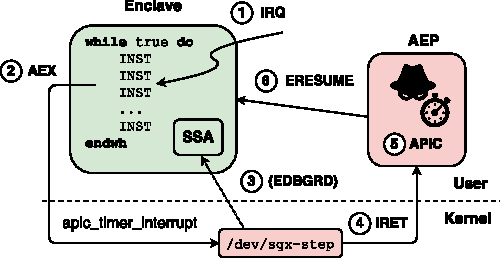
\includegraphics[width=0.7\textwidth]{images/sgx-step-overview.pdf}
  \caption{Overview of the SGX-Step attack \cite{BulckPS17}.}
  \label{fig:sgx-step}
\end{figure}

The overall process of SGX-Step is illustrated in Figure~\ref{fig:sgx-step} and
works as follows:
\begin{enumerate*}
  \item[\ding{172}]
    The enclave is interrupted by the APIC timer.
  \item[\ding{173}]
    The AEX procedure saves the enclave's state in the SSA and hands over
    control to the \texttt{/dev/sgx-step} kernel module.
  \item[\ding{174}]
    The kernel module reads the current instruction pointer of the enclave
    using the \textsc{edbgrd} instruction.
    This is meant for debugging and ensuring that the timer is configured
    correctly.
  \item[\ding{175}]
    The kernel module transfers control to the user space trampoline.
  \item[\ding{176}]
    From user space, the APIC timer is configured such that it interrupts the
    first instruction after the enclave is resumed.
  \item[\ding{177}]
    Resume the enclave with \textsc{eresume}.
\end{enumerate*}

One additional feature provided by SGX-Step is the monitoring of page table
entries.
Single-stepping the whole enclave can be quite sluggish.
It would be beneficial if it can be used for certain functions alone.
SGX-Step allows the attacker to start single-stepping once a specific code or
data page is accessed \cite{BulckWKPS17}.
It configures mappings between user space virtual memory and the physical
memory that houses the PTEs in the enclave.
Using the ``present'' bit to cause page faults \cite{XuCP15} or the
``accessed'' and ``dirty'' properties to reveal information about when a
specific function is called, an attacker can target specific areas they want to
single-step through.

The dangers of SGX-Step lie in its ability to amplify side-channel attacks.
By repeatedly interrupting the enclave after each instruction, the attacker can
gain information about a side-channel at maximal temporal resolution.
This has already been applied to various attack vectors, like extracting memory
access patterns through the cache side channel \cite{HahnelCP17}.

\subsection{CopyCat}

CopyCat \cite{MoghimiBHPS20} demonstrates the danger of single-stepping attacks
by utilizing SGX-Step to infer fine-grained control-flow information from SGX
enclaves.
It improves upon traditional page-fault adversaries, that can only observe page
accesses at a 4 KiB resolution, and uses single-stepping to capture control
flow at a maximum temporal resolution.
CopyCat has even been used to defeat a compiler hardening technique
\cite{HosseinzadehLLP18} that was suppose to withstand the SGX-Step attack.

We explain how CopyCat works using the example of square-and-multiply.
In a vulnerable square-and-multiply implementation, we can use page faults to
extract the key.
On each iteration we can induce a fault by clearing the execute permission on
the page with the \emph{square} function.
Tracking access in each iteration, we can fully recover the key from only page
faults.
Traditional page-fault adversaries fail at recovering the key when the entire
square-and-multiply procedure fits on a single page.
CopyCat overcomes this challenge by single-stepping the enclave and counting
the number of instructions until a data page was accessed.
By comparing the data access pattern with the function, CopyCat is able to
recover the key even if all used functions fit on a single page.

\begin{figure}[t!]
  \centering
  \includegraphics{square-and-multiply.pdf}
  \caption{A typical implementation of the exponentiation function using square and multiply.
    The function calculates $c^d$ where $c$ and $d$ are natural numbers.
    It is important to note that \emph{square} and \emph{multiply} are separate functions
    and may reside on different pages than the exponentiation function.}
  \label{fig:square-and-multiply}
\end{figure}

Figure~\ref{fig:square-and-multiply} illustrates the square-and-multiply
example.
The code fits on a single page,
but we still access the variables on a separate data page.
There are two data accesses of interest.
Therefore, we can observe code and data page accesses.
The first is the access to the output message $m$ that is squared on each
iteration.
The second is the access to the cipher text when we multiply $m$ by $c$.
This data access only happens when the key bit $d[i]$ equals one.
Hence, we will have three data accesses to $c$, $m$ and $d$ in one iteration,
while we will have only two accesses if the key bit is zero.
Therefore, by counting the number of instructions in each iteration,
CopyCat can recover the key even if the cipher text, output and key are on the
same page.

\subsection{AEX-Notify}
\label{sec:aex-notify}

To counter SGX-Step and the attack vectors that it enables, AEX-Notify has been
proposed.
The purpose of AEX-Notify is to stop attackers from reliably single-stepping an
enclave, which mitigates many attacks based on SGX-Step like CopyCat.

\begin{figure}
  \centering
  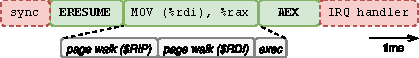
\includegraphics{images/sgx-step-without-prefetch.pdf}
  \caption{
    The main reason behind the effectiveness of SGX-Step is the assisted
    page-table walk \cite{ConstableBCXXAK23}.
    The \textsc{mov} instruction has to access the code page
    (\textsf{\itshape\$RIP}) and the memory location (\textsf{\itshape\$RDI}).
    The accessed bit has been cleared on both pages, causing a page walk for
    both accesses.}
  \label{fig:pte-walk}
\end{figure}

Constable et al. \cite{ConstableBCXXAK23} list the main reason behind the
effectiveness of SGX-Step as the assisted page-table walk, as shown in
Figure~\ref{fig:pte-walk}.
Before resuming the enclave, the attacker clears the ``accessed'' (A) bit on
the enclave's code page.
This forces the first instruction after \textsc{eresume}
to perform an expensive microcode assist to set the A-bit.
This induces additional latency in the execution of that instruction, because
the processor has to walk the page table again.
Thus, there is a large time frame where the interrupt of the timer could arrive
and land exactly on the first instruction.
The goal of AEX-Notify is to reduce the latency of the first instruction and
make it impossible to reliably land on the first instruction.

\begin{figure}[t]
  \centering
  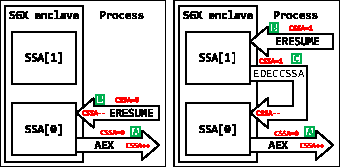
\includegraphics[width=0.6\textwidth]{images/sgx-ssa-edeccssa.pdf}
  \caption{
    Difference between the behavior of \textsc{eresume} when AEX-Notify is
    disabled (left) and when AEX-Notify is enabled (right).
    When AEX-Notify is enabled, an exception handler is executed with the top
    SSA \protect\greenbox{B}.
    The handler resumes the enclave with the new \textsc{edeccssa} instruction
    \protect\greenbox{C}, which decrements \textsc{cssa}.}
  \label{fig:aex-notify-edeccssa}
\end{figure}

\paragraph{Hardware Extension.}
The first part of AEX-Notify is the hardware extension.
It introduces a new flag in the SSA frame, called \textsc{aexnotify}.
Enabling this flag modifies the behavior of the \textsc{eresume} instruction.
Usually, \textsc{eresume} restores the previous process context, however, when
the \textsc{aexnotify} bit is enabled, a custom exception handler is executed.
The exception handler is responsible for handling the AEX and can afterwards
resume the enclave application with an additional instruction, called
\textsc{edeccssa}.
This instruction decrements the \textsc{tcs.cssa} field and restores the
context of the original enclave application.
Figure~\ref{fig:aex-notify-edeccssa} shows the difference between resuming an
enclave with and without AEX-Notify enabled.

\paragraph{Software Mitigation.}
The second part of AEX-Notify is the custom exception handler implemented in
software.
The handler runs after calling \textsc{eresume} and
uses the new \textsc{edeccssa} instruction to resume the enclave.
The exception handler's task is to prefetch the pages that the enclave accesses
during execution of the first instruction.
This process is split into two stages.

The first stage is responsible for decoding the first instruction and computing
a working set of the accessed pages from the first instruction.
This is done by decoding the first instruction and examining the saved SSA of
the enclave to retrieve potential memory locations.
The instruction decoder works in constant time \cite{TODO} such that it does
not leak any information about the instruction through timing attacks.
The working set is then passed to the second stage, where the memory locations
are prefetched to ensure that the first instruction can always be executed
quickly.
Before resuming the enclave, an additional delay of 20 cycles is inserted with
50 \% probability, making it even harder to reliably interrupt after the second
stage.


The first stage runs entirely with AEX-Notify disabled
and AEX-Notify is re-enabled during the second stage before prefetching the pages.
AEX-Notify is disabled at first to ensure that the exception handler always
makes forward progress.
However, it is re-enabled before prefetching to ensure that the pages are
\emph{always} prefetched before the enclave is resumed.

\section{Work Description}

Our main goal is to analyze the effectiveness of AEX-Notify
in preventing attackers from reliably single-stepping SGX enclaves.
To evaluate the success of AEX-Notify, we conducted an analysis aimed at
identifying any potential weak points in its implementation.
This section outlines the steps we took in our evaluation process,
beginning with the setup of the SGX-Step attack and
the subsequent enabling of AEX-Notify on this attacker.
By examining these components,
we aimed to provide an informed assessment of AEX-Notify’s defensive capabilities.
This analysis has informed us about potential attack vectors to try,
offering insights into areas that may require further study.

\subsection{Attacker Model}

In this project, we assume the standard Intel SGX privileged attacker model.
This means that the attacker has full control over the operating system
and can control important system functions.
For example, the attacker may modify the page-table to learn about memory accesses
or they may configure the APIC timer to interrupt the enclave, like SGX-Step.
This model is particularly relevant in scenarios such as cloud computing
environments, where cloud service providers could potentially exploit their
privileged access to the hardware and software stack to launch attacks against SGX enclaves.

\subsection{Initializing SGX-Step}

%\todo[inline]{Explain kernel module, \textsc{/dev/sgx-step}, etc.}

SGX-Step requires careful configuration of the APIC timer
since it is crucial for the attack to work.
If the value is too small, we will zero-step and execute the same instruction multiple times.
If the value is too large, we will multi-step and execute multiple instructions.
We have used the benchmark application provided in the SGX-Step repository for this purpose.
The program consists only of a series of \textsc{nop} instructions and
reports the instruction pointer after each interrupt using the \textsc{edbgrd} instruction.
If the instruction pointer is incremented by one instruction each interrupt,
then we can be sure that we are single-stepping and
that we have configured SGX-Step correctly.

% TODO: Make clear that this is the victim, which we will use for testing purposes

\subsection{Enabling AEX-Notify}

After configuring SGX-Step and successfully single-stepping the enclave, we
enabled AEX-Notify.
We have enabled AEX-Notify by simply adding an additional field in the enclave
configuration file.
Enabling this flag technically requires registering an exception handler that
handles any enclave exits.
However, the exception handler is preconfigured to use the provided handler
from the trusted runtime system of the Intel SGX SDK.
This is the exact same exception handler as described in
Section~\ref{sec:aex-notify}, which decodes the first instruction from the
enclave and prefetches the necessary code and data pages.

\subsection{Analyzing AEX-Notify}

After enabling AEX-Notify, we verified that we can no longer single-step the
enclave by comparing the reported addresses from a previous run.
Usually, we can use these addresses to configure the timer since each address
is incremented by one when the timer is configured correctly.
The problem with AEX-Notify is that interrupting the enclave not only
interrupts the enclave but it can also interrupt the exception handler.
Hence, the application will additionally report addresses from the exception
handler.

For these addresses, it is not entirely clear where exactly they are located in
the source code.
In debug mode, the instruction pointer can help identify these addresses.
Therefore, we have written a simple tool that uses the debug information from
the binary and automatically translates these addresses to their source code
location in the trusted runtime system.

The overall analysis has lead us to an important question regarding the
exception handler:
whether interrupting the exception handler during the second stage would
restart the entire exception handler again or only restart the second stage.
If an interrupt during the second stage would only restart the second stage,
then we could effectively differentiate between a zero and a multi-step.

We have analyzed this potential weak point by modifying the second stage to
cause an interrupt.
This involved adding one additional instruction in the second stage.
This instruction would access a page that the enclave has no read permission for.
Hence, a page fault occurs and the enclave is interrupted during the second stage.
The last step is recognizing where this interrupt is handled.
To achieve this, we induce another page fault on the first stage of the exception handler
and we check whether another page fault occurs immediately after the first.

\subsection{Simulating a Cache Attack}

Our assumption is that we are able to detect when the last page access occurs
during the second stage of the exception handler.
The idea would be that one would use a side-channel, like a cache attack, to
detect when this happens.
We simulate such an attack by incrementing a variable that is shared between
the enclave and the attacker.
We have modified the exception handler such that it increments the shared
variable once the second stage is finished.
The attacker can then monitor this variable for any changes.
Once the variable is incremented, the attacker reconfigures the APIC timer to
immediately interrupt the enclave again.
The goal of this attack is to see whether it is possible to distinguish between
zero-stepping and multi-stepping.

After incrementing the variable, the exception handler inserts a random delay
before resuming the enclave.
The delay may cause our second interrupt -- the one after the simulated cache
access -- to interrupt the exception handler and not the enclave.
This would cause us to zero-step instead of multi-stepping.
Therefore, we'll have to be able to distinguish zero-stepping from
multi-stepping for our attack to be effective.

We have introduced a second counter to help test our multi-stepping attack.
This counter is incremented after each instruction from the victim code,
which essentially forms another instruction pointer.
This instruction pointer tells us how far the enclave has advanced.
This counter is only for testing the effectiveness of our attack
and is not used inside the attack itself.

\section{Results}

\paragraph{Single-Stepping Resilience.}
As the most basic requirement,
we were no longer able to single-step the enclave after enabling AEX-Notify.
We were always able to reliably interrupt the application
before executing the first instruction of the target code
by using the additional page-fault side channel provided by SGX-Step.
However, we were unable to reliably execute one or
even multiple instructions after executing the first.
The first instruction is no longer artificially prolonged,
and there is now a random delay in the interrupt handler.
Without these two measures,
it would still be possible to configure a timer interval
that could skip over the exception handler and land directly on the first instruction.

Since the application reports the instruction pointer of the enclave,
we could see that the addresses no longer correspond to only our target.
Instead, most of these addresses pointed to the exception handler.
Between these addresses, sometimes the program would report addresses from our target.
However, the addresses always jumped at least several instructions from the previous
and we were never able to reliably cause a controlled multi-step attack
by only configuring the APIC timer.

\paragraph{Interrupting the Exception Handler.}
We were able to verify that the exception handler is always rolled back to the
first phase of the exception handler.
This is still the case, even if we interrupt the second stage, where AEX-Notify
is re-enabled.
By inserting a page-fault after the assembly stub re-enables AEX-Notify, we
were able to detect that the exception handler is reset completely, i.e. it
starts from the first phase.
This ensures that an attacker cannot simply interrupt the exception handler
to differentiate between a zero-step and a multi-step,
showing the security of AEX-Notify.

\paragraph{Simulated Cache Attack.}

As an alternative, we have induced a page fault on the counter page to
interrupt the enclave.
Although this did successfully interrupt our enclave, it would usually take
more than $5\,000$ instructions until the interrupt arrived.
Such a large time frame defeats the purpose of multi-stepping using interrupts
since a regular page-fault adversary can already leak control-flow information
at a 4 KiB (spatial) granularity \cite{TODO}.

\section{Conclusion and Future Work}

With this study, we explored the functionality of AEX-Notify in Intel SGX and
its effectiveness in preventing single-stepping attacks.
Our experiments showed that once AEX-Notify is enabled, single-stepping attacks
become significantly more difficult, strengthening the argument that AEX-Notify
is effective in mitigating such attacks.

In conclusion, our findings suggest that AEX-Notify is a promising feature for
enhancing SGX security, but additional testing is necessary to confirm its
effectiveness against a wider range of attacks.

\bibliographystyle{alpha}
%\bibliographystyle{splncs03}
\bibliography{references}

\clearpage
\appendix

\section{Modified Second Stage of the AEX-Notify Exception Handler}

The following code lists the second stage of the exception handler from AEX-Notify \cite{ConstableBCXXAK23},
where the code and data pages are prefetched.
Our modification (highlighted in green) increments a counter shared between the enclave and attacker.
The counter's address is loaded into \textsc{rcx} and incremented, but only if it is not null to prevent null pointer dereferencing.

\noindent
\rule{0.8\textwidth}{0.4pt}
\vspace{-0.5em}
\lstinputlisting[style=code,lastline=47]{trts_mitigation_modified.S}%
\vspace{-1.1em}
\lstinputlisting[firstnumber=48, firstline=48,lastline=52, basicstyle=\ttfamily\scriptsize\bfseries\color{green!50!black}]{trts_mitigation_modified.S}%
\vspace{-1.1em}
\lstinputlisting[style=code,firstnumber=53, firstline=53]{trts_mitigation_modified.S}
\vspace{-1em}
\rule{0.8\textwidth}{0.4pt}

\end{document}
